\documentclass{beamer}

\mode<presentation>
{
  \usetheme{Warsaw}      
  \usecolortheme{crane} 
  \usefonttheme{default}  
  \setbeamertemplate{navigation symbols}{}
  \setbeamertemplate{caption}[numbered]
} 

\usepackage[english,serbian]{babel}
\usepackage[utf8]{inputenc}
\usepackage[T2A]{fontenc} 
\usepackage{currvita}
\usepackage{listings}
\usepackage{lipsum}

\title[Klasifikacija oročenog depozita]{Analiza skupa Bank Customer Survey – Marketing for Term Deposit metodom klasifikacije}%short, full
\author[Tamara Ivanović]{Tamara Ivanović, 462/2018}
\institute{\small{Seminarski rad u okviru kursa\\Istraživanje podataka 1\\ Matematički fakultet}}
\date{Avgust, 2019.}

\begin{document}

\begin{frame}
  \titlepage
\end{frame}



%%%%%%%%%%%%%%%%%%%%%%%%%%%%%%%%%%
\section{Uvod}

\begin{frame}{Uvod}

\begin{itemize}
  \item Klasifikacija skupa bank marketing term deposit 
  \item Analiza i pretprocesiranje
  \item Klasifikacija u SPSS modeleru
  \item Klasifikacija u Pythonu
  \item Analiza dobijenih modela
\end{itemize}

\end{frame}

%%%%%%%%%%%%%%%%%%%%%%%%%%%%%%%%%%
\section{Analiza i pretprocesiranje}
\subsection{Lista atributa}
\begin{frame}{Lista atributa}
	\begin{figure}[h!]
                \begin{center}
                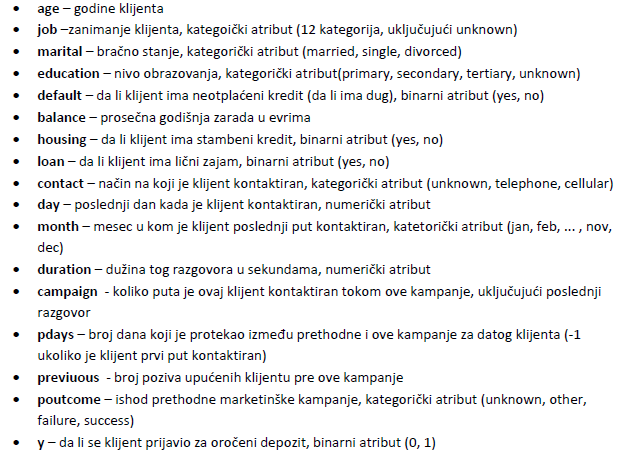
\includegraphics[scale=0.60]{atributi.png}
                \end{center}
                \caption{Atributi skupa}
     \end{figure}
    
\end{frame}

%%%%%%%%%
\subsection{Pretprocesiranje u Python-u}
\begin{frame}{Pretprocesiranje u Python-u}
    	\begin{itemize}
		\item Nema \textit{null} vrednosti
		\item \textit{unknown} zamenjeno kod \textit{education} i \textit{job}		
		\item Uklonjeni atributi \textit{poutcome}, \textit{contact} i \textit{day}
		\item MinMaxScaler(), train\_test\_split()
		
		% slika za skriptovanje
		\begin{figure}[h!]
                \begin{center}
                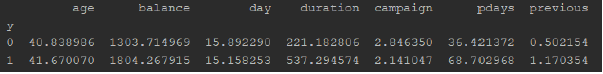
\includegraphics[scale=0.70]{prosecne_vrednosti.png}
                \end{center}
                \caption{Prosečne vrednosti atributa}
                \label{fig:prosecne_vrednosti}
         \end{figure}
		
		\item \textit{duration, pdays, previous, campaign, balance, job, education}
	\end{itemize}	
\end{frame}

\begin{frame}{Pretprocesiranje u Python-u}
    	
		
		% slika za korelacije
		\begin{figure}[h!]
                \begin{center}
                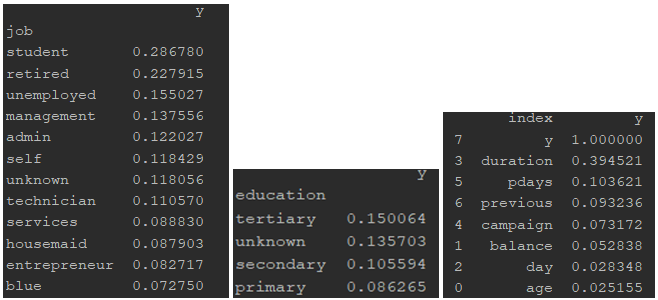
\includegraphics[scale=0.50]{korelacije.png}
                \end{center}
                \caption{Korelacije atributa}
                \label{fig:korelacije}
         \end{figure}
		
			
\end{frame}

%%%%%%%%%%%%
\subsection{Pretprocesiranje u SPSS modeleru}
\begin{frame}{Pretprocesiranje u SPSS modeleru}
  			\begin{figure}[h!]
                \begin{center}
                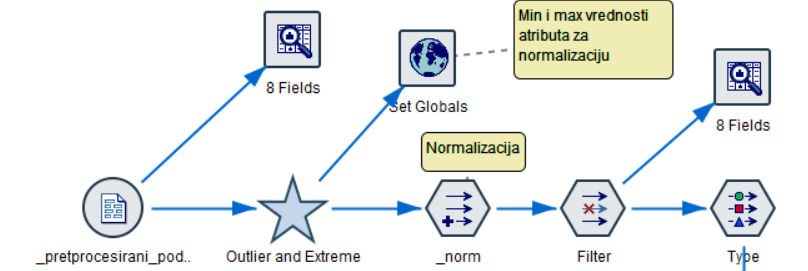
\includegraphics[scale=0.60]{pretprocesiranje_SPSS.png}
                \end{center}
                \caption{Shema pretprocesiranje u SPSS modeleru}
                \label{fig:pretprocesiranje_spss}
             \end{figure}
\end{frame}
%%%%%%%%%%%%%%%%%%%%%%%%%%%%%%%%%%%%%%%%%%%%%%%%%%%%%%%%%%
\section{Klasifikacija}
\begin{frame}{Klasifikacija}
    \begin{itemize}
        \item C5.0
        \item CART
        \item KNN
        \item QUEST
        \item Bajesove mreže
        \item Naivan Bajesov algoritam
    \end{itemize}
\end{frame}

%%%%%%%%%%%%%%%%%%
\subsection{C5.0}
\begin{frame}{C5.0}

	 \begin{itemize}
        \item Drvo odlučivanja
        \item Tendencija je preciznost
        \item Dubina 13
    \end{itemize}
    \begin{figure}[h!]
                \begin{center}
                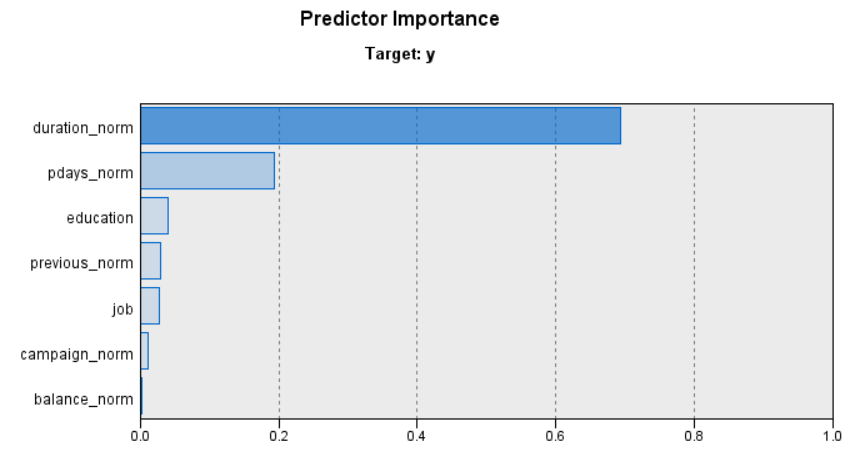
\includegraphics[scale=0.4]{c5_predictor.png}
                \end{center}
                \caption{Algoritam C5.0 - Važnost prediktora}
             \end{figure}
\end{frame}

\begin{frame}{C5.0}
    \begin{figure}[h!]
                \begin{center}
                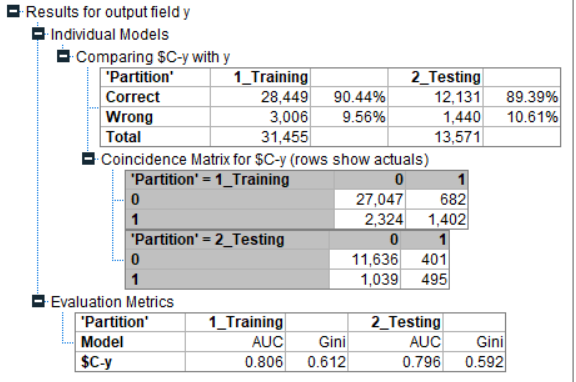
\includegraphics[scale=0.60]{c5_matrix.png}
                \end{center}
                \caption{Algoritam C5.0 - Matrica konfuzije}
             \end{figure}
\end{frame}
%%%%%%%%%%%%%%%%%%
\subsection{CART}

\begin{frame}{CART}
	 \begin{itemize}
        \item Minimalna dubina stabla: 4
        \item Ginijev indeks
        \item Bolja stabilnost - Enhance model stability
		\item Potrkesivanje stabla radi izbegavanja preprilagođenosti        
    \end{itemize}
    \begin{figure}[h!]
                \begin{center}
                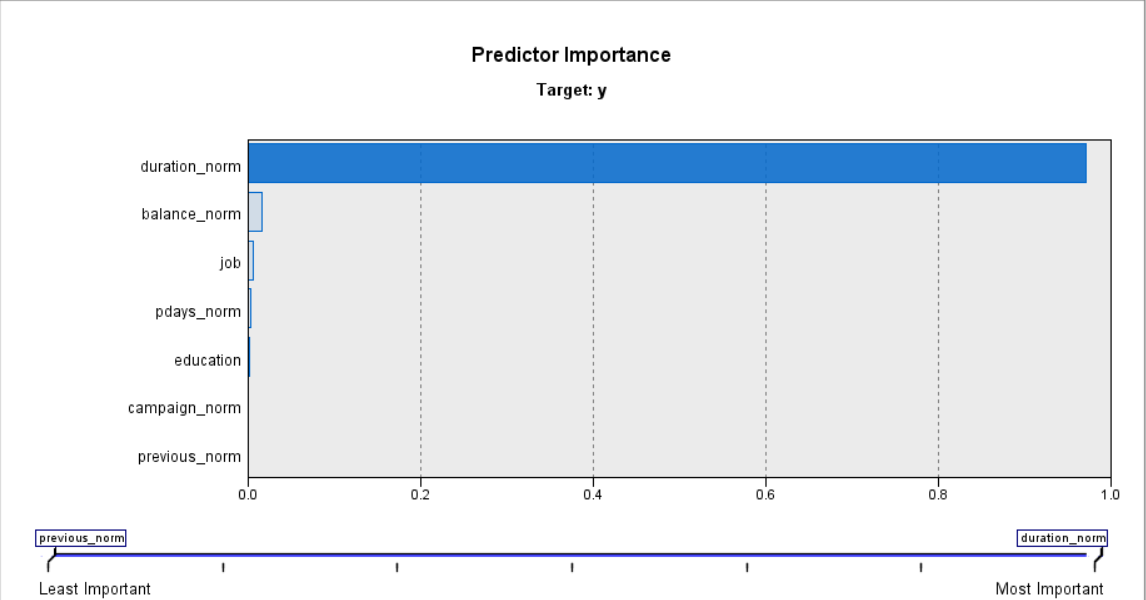
\includegraphics[scale=0.30]{cart_predictor.png}
                \end{center}
                \caption{Algoritam CART - Važnost prediktora}
             \end{figure}
\end{frame}

\begin{frame}{CART}
    \begin{figure}[h!]
                \begin{center}
                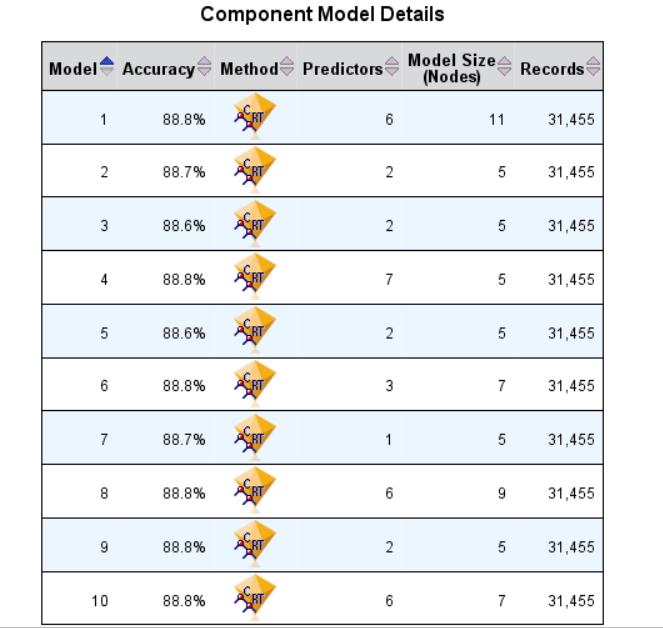
\includegraphics[scale=0.40]{cart_component_model.png}
                \end{center}
                \caption{Algoritam CART - Modeli}
             \end{figure}
\end{frame}

\begin{frame}{CART}
    \begin{figure}[h!]
                \begin{center}
                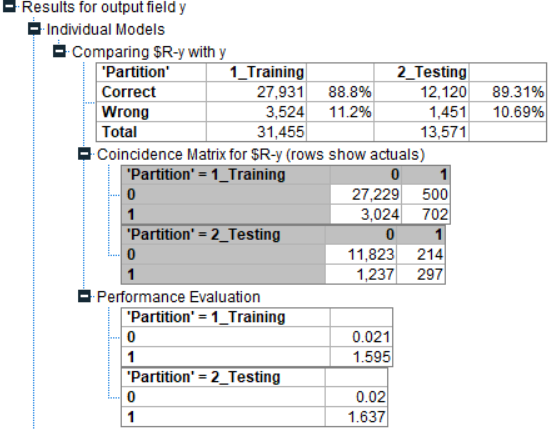
\includegraphics[scale=0.60]{cart_matrix.png}
                \end{center}
                \caption{Algoritam CART - Matrica konfuzije}
             \end{figure}
\end{frame}

%%%%%%%%%%%%%%%%%%
\subsection{KNN}

\begin{frame}{KNN}
    \begin{itemize}
        \item Cilj: Preciznost modela
        \item k između 3 i 8
        \item Menhetn rastojanje
        \item Prediktori jednako važni
        \item Za k=6 i k=8 najbolja rešenja
    \end{itemize}
\end{frame}

\begin{frame}{KNN}
    \begin{figure}[h!]
                \begin{center}
                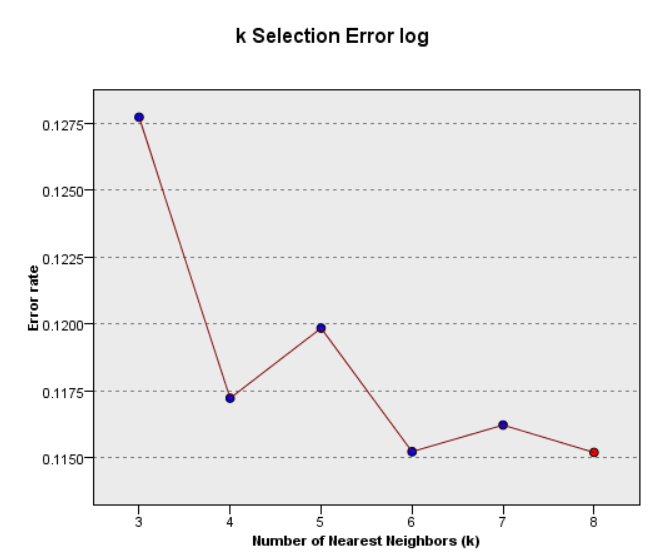
\includegraphics[scale=0.50]{knn_error.png}
                \end{center}
                \caption{Algoritam KNN - Nivo greške u zavisnosti od k}
             \end{figure}
\end{frame}

\begin{frame}{KNN}
    \begin{figure}[h!]
                \begin{center}
                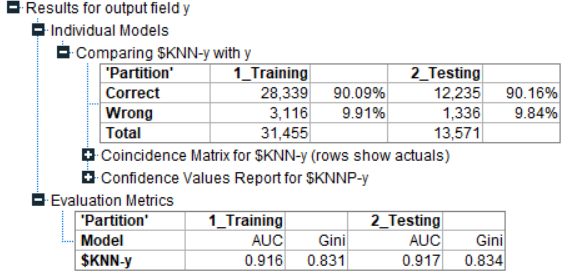
\includegraphics[scale=0.60]{knn_matrix.png}
                \end{center}
                \caption{Algoritam KNN - Matrica konfuzije}
             \end{figure}
\end{frame}

%%%%%%%%%%%%%%%%%%
\subsection{QUEST}
\begin{frame}{QUEST}
    \begin{itemize}
        \item Binarno stablo
        \item Uvek dubina 2
        \item \textit{duration} najbitniji 
        \item Ostali prediktori jednako važni, ali zanemarljivi
        \item AUC = 0.637, blizu 0.5
    \end{itemize}
\end{frame}

\begin{frame}{QUEST}
    \begin{figure}[h!]
                \begin{center}
                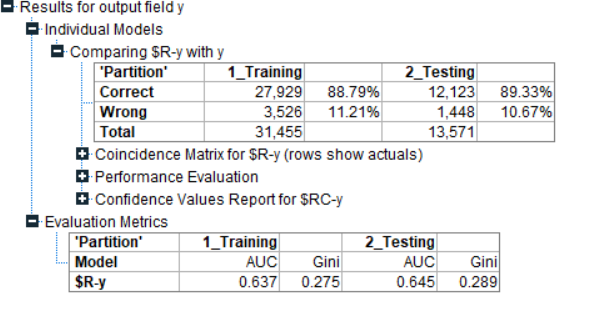
\includegraphics[scale=0.60]{quest_matrix.png}
                \end{center}
                \caption{Algoritam QUEST - Matrica konfuzije}
     \end{figure}
\end{frame}

%%%%%%%%%%%%%%%%%%
\subsection{Bajesove mreže}

\begin{frame}{Bajesove mreže}
    \begin{itemize}
        \item Bajesova statistika
        \item Posmatra \textit{duration}, zatim \textit{job}
        \item Uslovne verovatnoće svake instance
        \begin{figure}[h!]
                \begin{center}
                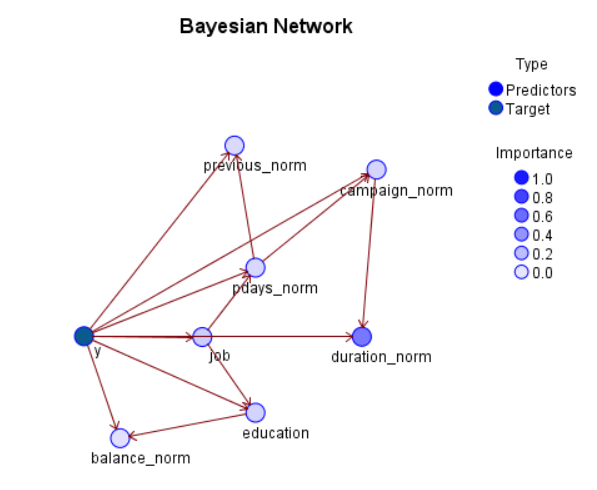
\includegraphics[scale=0.40]{Bajes_mreza.png}
                \end{center}
                \caption{Algoritam Bajesove mreže}
     	\end{figure}
    \end{itemize}
\end{frame}

\begin{frame}{Bajesove mreže}
    \begin{figure}[h!]
                \begin{center}
                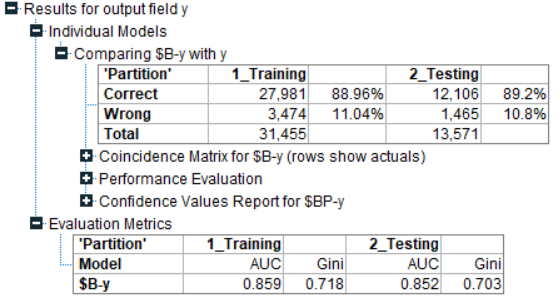
\includegraphics[scale=0.60]{Bajes_matrix.png}
                \end{center}
                \caption{Algoritam Bajesove mreže - Matrica konfuzije}
     \end{figure}
\end{frame}

%%%%%%%%%%%%%%%%%%
\subsection{Naivan Bajesov algoritam}

\begin{frame}{Naivan Bajesov algoritam}
    \begin{itemize}
    	\item trening skup 0,75, test skup 0,25
        \item 1-yes, 0-no
        \item sklearn.naive\_bayes
        \item Gausova formula 
    \end{itemize}
\end{frame}

\begin{frame}{Naivan Bajesov algoritam}
    \begin{figure}[h!]
                \begin{center}
                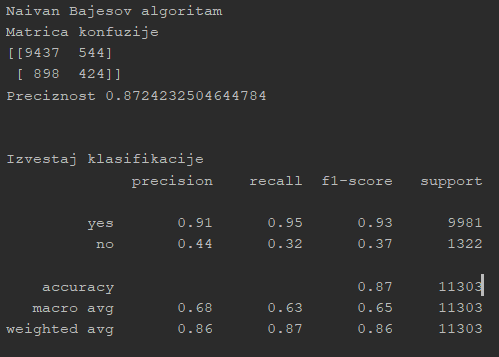
\includegraphics[scale=0.60]{naive_B_matrix.png}
                \end{center}
                \caption{Naivan Bajesov algoritam - Matrica konfuzije}
     \end{figure}
\end{frame}
%%%%%%%%%%%%%%%%%%%%%%%%%%%%%%%%%%%%%%%%%
\section{Zaključak}
\begin{frame}{Zaključak}
    \begin{figure}[h!]
                \begin{center}
                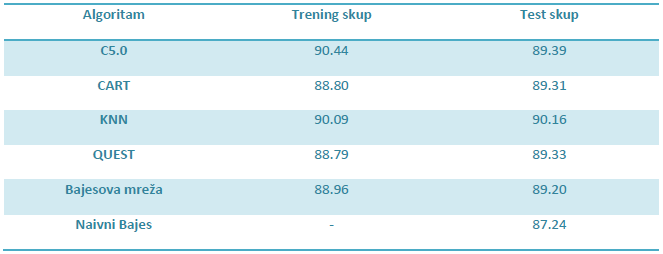
\includegraphics[scale=0.60]{zakljucak.png}
                \end{center}
                \caption{Preciznost algoritama}
      \end{figure}
\end{frame}


\begin{frame}{}
    \begin{center}
    Hvala na pažnji!
    \end{center}
\end{frame}
%%%%%%%%%%%%%%%%%%%%%%%%%%%%%%%%%%%%%%%%%


\end{document}






